\section{Conclusion}\label{conclusion}


\paragraph{}

Au moment où ce rapport a été rendu, ce travail n'était plus qu'à une étape d'aboutir:
la démarche d'approximation des fenêtres duales $\h{\t{w}}$ est validée numériquement par \ref{implementation},
avec l'indication des paramètres à choisir pour obtenir les résultats souhaités pour une bonne reconstruction de $\v{E}$:

\subparagraph{}

Pour une précision de $\eepsilon=10^{-3}$, une longueur d'onde $\lambda_0=1m$, une largeur de fenêtre $L_x=8\lambda_0$,
et surtout un coefficient du suréchantillonnage $\nu_x=0.25$, le programme Python associé à ce travail est capable
de calculer les coefficients $(A_{m,n,p,q})$ pour un nombre de termes assez significatif pour reconstruire correctement
le champ global. Une simulation prenant un temps de calcul d'au moins une demi-journée pour l'ordre $0$ d'approximation,
ce rapport ne comportera pas les résultats finaux de cette recomposition.
Ceux-ci seront surement disponibles juste après, dans un mail complémentaire ultérieur.


\paragraph{}

Cependant, la lecture de \cite{TheseLugara}, de \cite{TheseGhannoum}, ainsi que les résultats suivants,
trouvés avec des paramètres assez faibles pour que le programme s'exécute (mais trop faibles pour avoir un sens physique),
nous encourage à penser qu'il aurait suffit d'un peu plus de temps (ou d'un binôme sachant programmer un peu mieux)
pour optimiser le programme à temps et obtenir la reconstruction du champ électromagnétique global dans le temps imparti.
\footnote{Ces figures ne comportent pas d'échelle d'amplitude des champs, mais cela a été corrigé dans le script final.}

\subparagraph{}

\begin{figure}[h]
 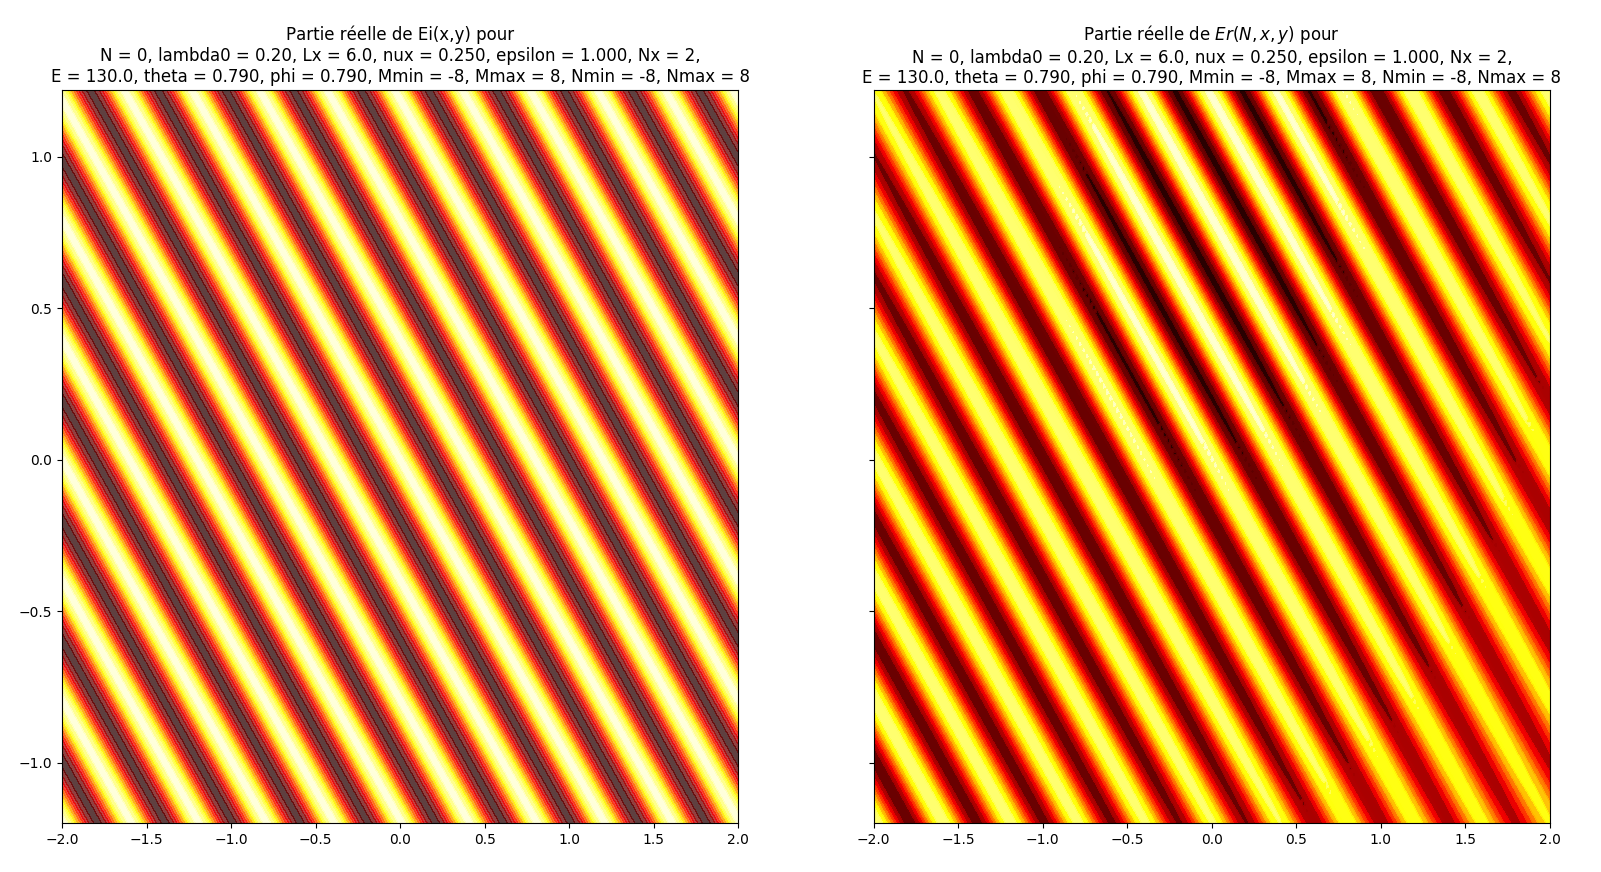
\includegraphics[scale=0.4]{hope.png}
\end{figure}




\newpage